\documentclass[a4paper,11pt]{article}

\usepackage[english,greek]{babel}

\newcommand{\lt}{\latintext}
\newcommand{\gt}{\greektext}

\usepackage{amsmath}
\usepackage[pdftex]{graphicx}
\usepackage{verbatim}  
\usepackage[section] {placeins}
\usepackage{multirow}
\usepackage{graphicx}

\title{1η Υποχρεωτική Εργασία \\ Στο Μάθημα της Αριθμητικής Ανάλυσης}
\author{Όνοματεπώνυμο: Γεώργιος Κεσογλίδης  \\  ΑΕΜ: 3911}
\date{\today} 

\begin{document}

\maketitle
\normalsize{
H υλοποίηση όλων των ασκήσεων πραγματοποιήθηκε στην \lt python.}

\section{Άσκηση 1}
\vspace*{0 cm}
\normalsize{
Σχεδιάζουμε την γραφική παράσταση με χρήση του \lt gnuplot:}
\\
\hspace*{-1 cm}
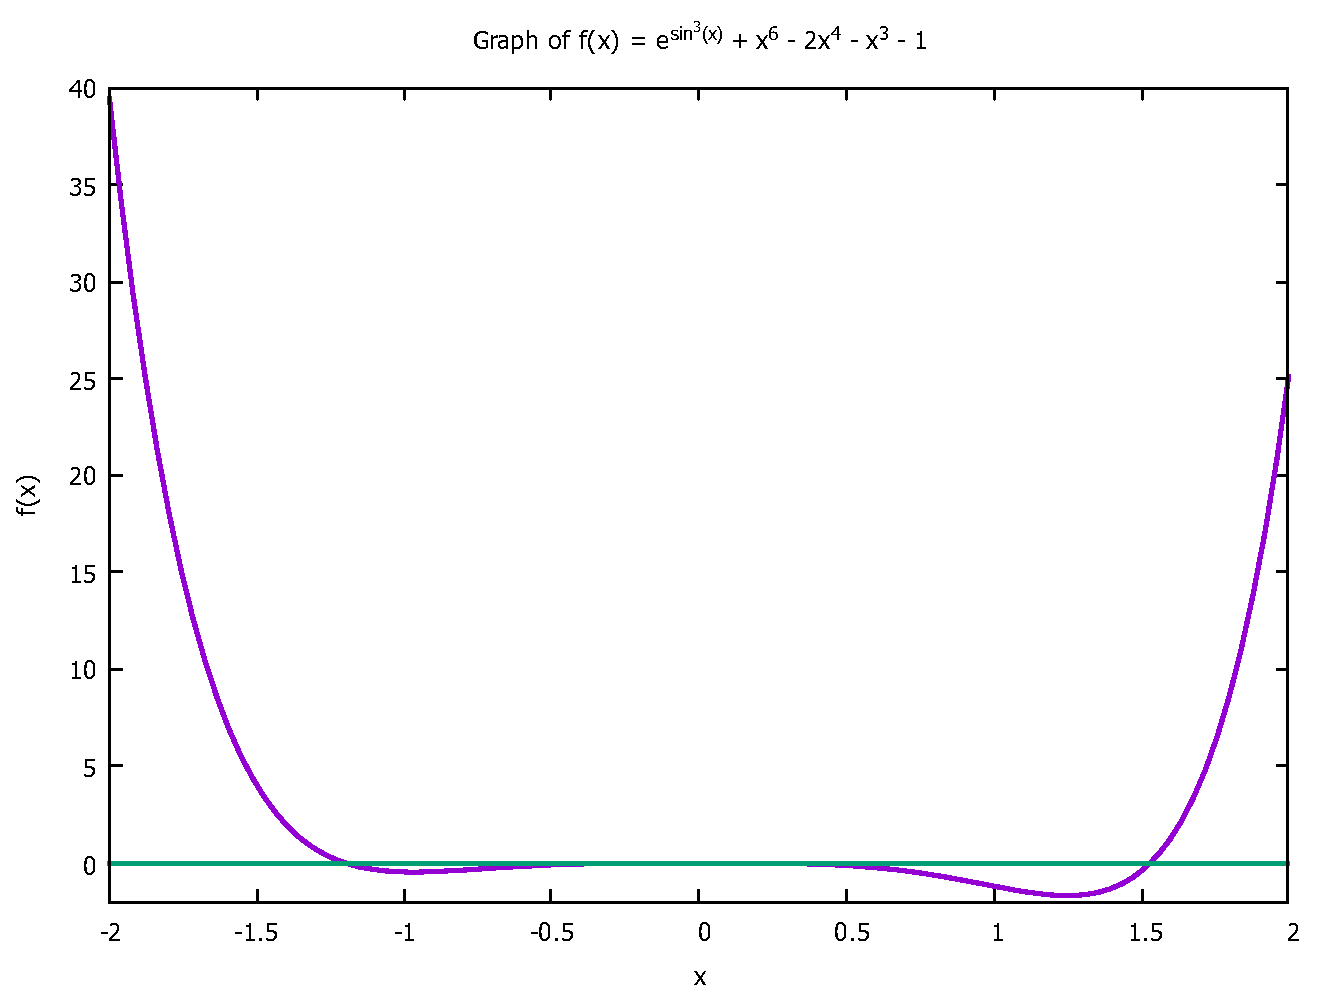
\includegraphics[height=12cm, width=15cm]{Ask1.pdf}
\newpage
\normalsize{	Για την συνάρτηση  \lt f(x) \gt εύκολα 	
υπολογίζεται ότι έχει ρίζα στο \lt x = 0. \gt 
\\ Επίσης, από το παραπάνω
γράφημα βλέπουμε ότι έχει μόνο αλλές δύο ρίζες κόντα στο \lt x = 1.5
\gt και στο \lt x = - 1.25. \gt Θα υπολογίσουμε αύτες τις ρίζες με
ακρίβεια πέντε δεκαδικών ψηφίων χρησιμοποιώντας τρεις διαφορετικές
\\επαναληπτικές μεθόδους. Για τον υπολογισμό εκθετικών και
τριγωνομετρικών συναρτήσεων χρησιμοποιούμε την βιβλιοθήκη \lt numpy.}

	\subsection{Μέθοδος της διχοτόμησης}
\normalsize{
Για την μέθοδο της διχοτόμησης θα επιλέξουμε τα διαστήματα [-2,-1] \\ 
και  [1, 2]. Από την γραφική παράσταση επιβεβαιώνουμε ότι ισχύουν οι 
\\ προύποθεσεις του Θεωρήματος \lt Bolzano. \gt Δηλαδή, ότι η
συνάρτηση είναι 
\\ συνεχείς και έχει ετερόσημες τιμές στα άκρα των διαστημάτων που
 αναφέραμε. Δεν
μπορούμε να εντοπίσουμε ότι η συνάρτηση έχει ρίζα στο 
\lt x = 0 \gt γιατί δεν έχει ετερόσημες τιμές κοντά της. 
\\Τα αποτελέσματα του προγράμματος είναι τα εξής: 
\par\lt For the interval [-2,-1] bisection loops 17 times 
\par and the root is -1.1976242065429688
\par For the interval [ 1, 2] bisection loops 17 times 
\par and the root is 1.5301284790039062}

	\subsection{Μέθοδος \lt Newton-Raphson}
\normalsize{Για την μέθοδο \lt Newton-Raphson \gt θα πάρουμε
ως αρχική τιμή πρώτα \\ \lt x =  -1.75 \gt , μετά \lt x = 0.3 \gt 
και τέλος \lt x = 1.75. \gt Μπορούμε να διαλέξουμε αυτές τις αρχικές
τιμές διότι η συνάρτηση κοντά στο \lt x = 0.3 \gt είναι αρνητική και
\\κοίλη ενώ για τις αλλές είναι θετική και κυρτή, 
άρα για όλες ισχύει}
\\
\begin{equation*}
	f(x_0)f"(x_0) > 0
\end{equation*}
\\
\normalsize{ Επίσης, από την θεωρία γνωρίζουμε ότι η
μέθοδος \lt Newton-Raphson \gt συγκλίνει τετραγωνικά για τις ρίζες
που η πρώτη και δεύτερη παράγωγος δεν μηδενίζονται για κάποιο
διάστημα που περιέχει την ρίζα και την αρχική τιμή. Από την γραφική
παράσταση της \lt f \gt παρατηρούμε ότι αυτό δεν ισχύει για την \lt 
\\ x = 0 \gt διότι είναι τοπικό μέγιστο και άρα έχει παράγωγο 0. Ενώ
για τις άλλες ρίζες υπάρχουν διαστήματα που δεν έχουν ούτε σημεία
καμπής ούτε τοπικά \\ ακρότατα οπότε συγκλίνουν τετραγώνικα.
Περιμένουμε η ακρίβεια να \\επιτευχθεί πολύ πιο αργά για \lt x = 0. 
\gt \\Τα αποτελέσματα του προγράμματος είναι τα εξής: 
\par\lt For x = -1.75 Newton-Raphson loops 7 times 
\par and the root is -1.1976237221338035
\par For x =  0.3 Newton-Raphson loops 30 times 
\par and the root is 8.576575582112126e-05
\par For x =  1.75 Newton-Raphson loops 5 times 
\par and the root is 1.5301335081746195
\\
\\ \gt Να τονίσουμε ότι από εδώ και πέρα, για να αποφύγουμε τον
υπολογισμό της παραγώγου με το χέρι, Θα χρησιμοποιούμε
τον συμμετρικό ορισμό της παραγώγου, δηλαδή 
\begin{equation*}
	f'(x) \approx \frac{f(x+h)-f(x-h)}{2h}
\end{equation*} 
για \lt h \gt που είναι ίσο με το σφαλμά μας ώστε να
μην επηρεάσει την εύρεση λύσης. Συγκεκριμένα 
\begin{equation*}
	h = 10^{-5}
\end{equation*}}

	\subsection{Μέθοδος της τέμνουσας}
		\normalsize{Η μέθοδος της τέμνουσας απαίτει τις ίδιες
προϋποθέσεις με την μέθοδο \lt Newton-Raphson. \gt Για ευκολία κάθε
\lt x0 \gt πού θα χρησιμοποιήσουμε θα είναι από τις \\παραπάνω
αρχικές τιμές και για \lt x1 \gt θα πάρουμε κάποιο κοντινό αριθμό που
\\ τηρεί τις ίδιες προϋποθέσεις. Θα πάρουμε λοιπόν πρώτα 
\lt x0 = -1.75, x1 = 2, \gt μετά \lt x0 = 0.3, x1 = 0.5 \gt 
και τέλος \lt x0 = 1.75, x1 = 2. \gt \\
Τα αποτελέσματα του προγράμματος είναι τα εξής: \par\lt
\par For x0 = -1.75 and x1 = -2 secant loops 10 times 
\par and the root is -1.1976237221353676
\par For x0 = 0.3 and x1 = 0.5 secant loops 41 times 
\par and the root is 9.870092240214844e-05
\par For x0 =  1.75 and x1 =  2 secant loops 7 times 
\par and the root is 1.5301335086057053}
		
\vspace*{7 cm}
\section{Άσκηση 2}
	\subsection{Ρίζες \lt f(x)}

	\normalsize{Σχεδιάζουμε την γραφική παράσταση της συνάρτησης 
	ώστε να δούμε περίπου που βρίσκονται οι ρίζες}
	\\
	\hspace*{-1 cm}
	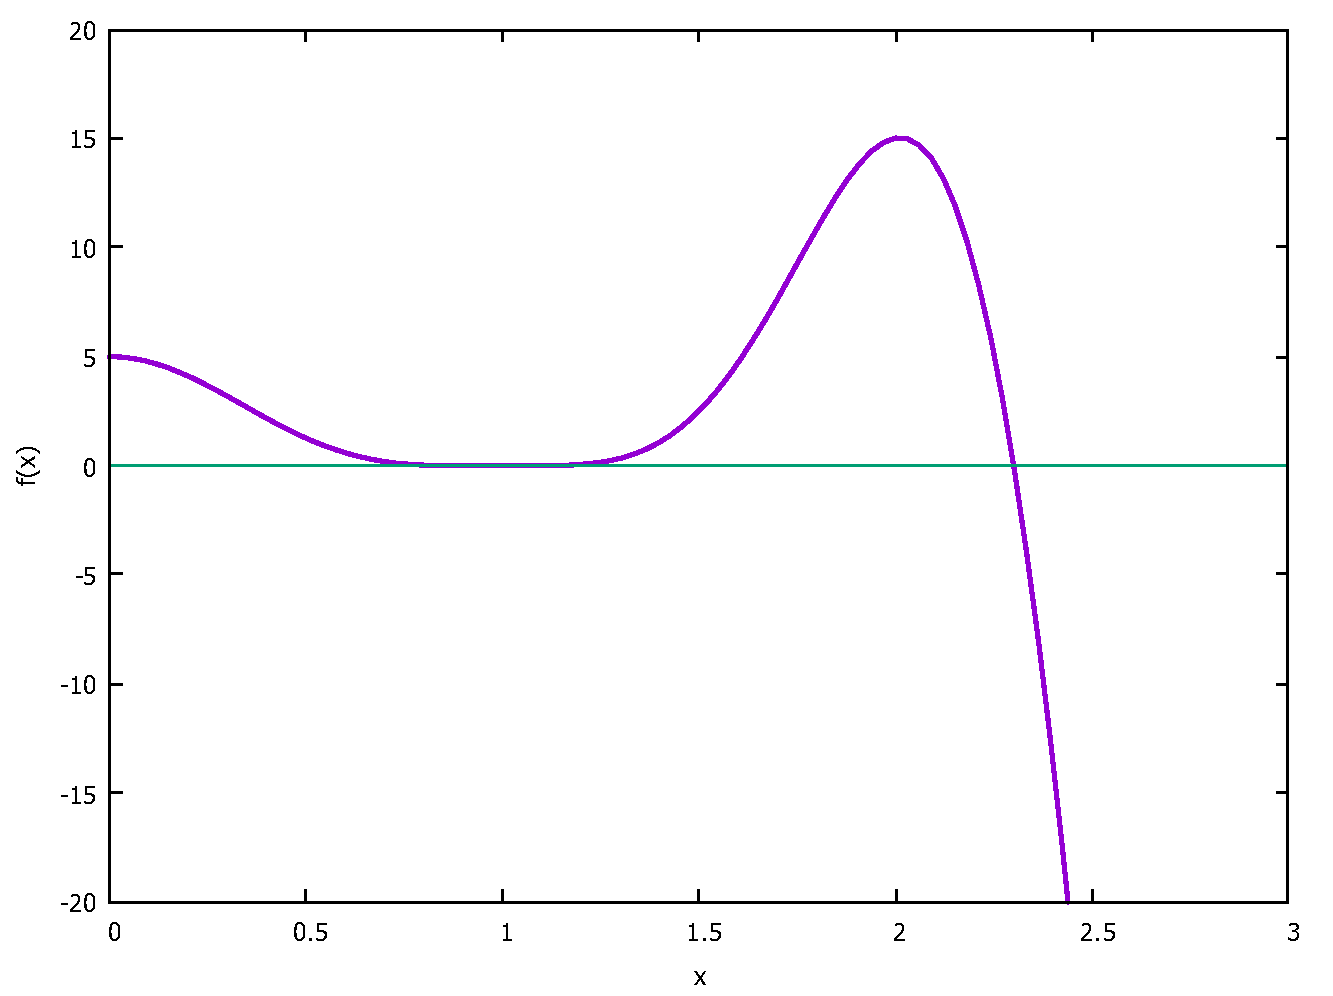
\includegraphics[height=8cm, width=15cm]{Ask2.pdf}
	\normalsize{Δεν φαίνεται καθαρά τι γίνεται κοντά στο 1 οπότε
 μεγενθύνουμε την γραφική παράσταση}	
	\\
	\hspace*{-2 cm}
	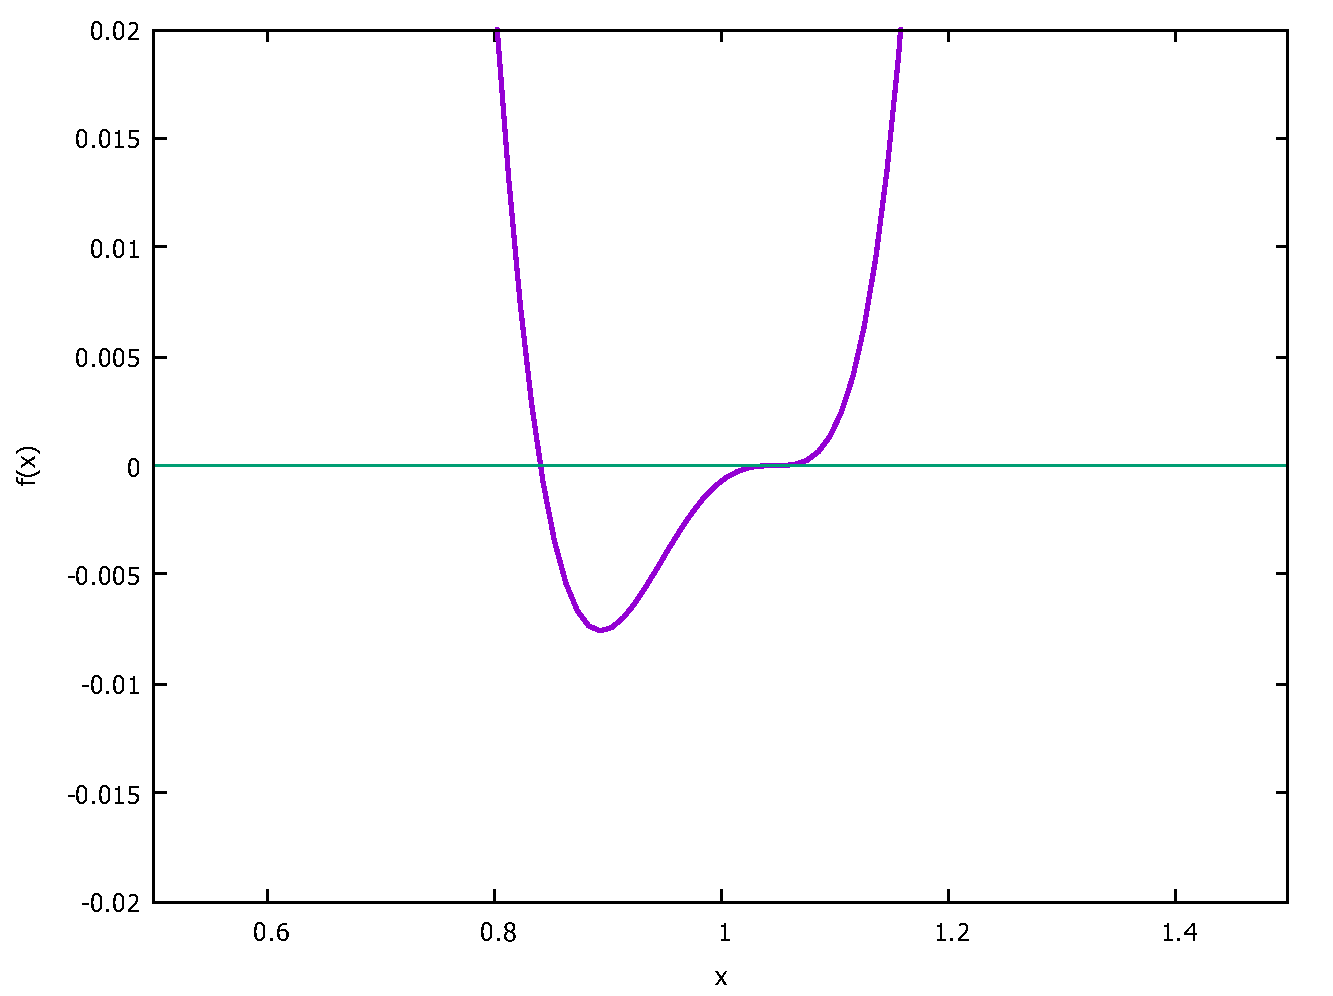
\includegraphics[height=8cm, width=16cm]{detail.pdf}
	\normalsize{Βλέπουμε οτι η \lt f \gt έχει τρεις ρίζες και 
	τώρα θα τις υπολογίσουμε}
	
	\subsubsection{Τροποποιήμενη μέθοδος \lt Newton-Raphson
	 \gt \\ Μέθοδος \lt Halley}
\normalsize{Για να αποφύγουμε διαίρεση με πολύ μικρό αριθμό θα 
γράψουμε τον τύπο ως εξής:}
\\
\begin{equation*}
	x_{n+1} = x_n - \frac{1}{\frac{f'(x_n)}{f(x_n)}-\frac{1}{2}
\frac{f"(x_n)}{f(x_n)}} => x_{n+1} =
\frac{2f(x_n)f'(x_n)}{2f^2(x_n)-f(x_n)f"(x_n)}
\end{equation*}
\\
\normalsize{Διαλέγουμε \lt x = 0.5\gt , μετά \lt x = 1 \gt  
και τέλος \lt x = 2.5 \gt επειδή ικανοποιούν τα κριτήρια 
που προαναφέρθηκαν στην 1.2. \\
Τα αποτελέσματα του προγράμματος είναι τα εξής:
\par\lt	For x = 0.5 Halley loops 5 times 	
\par and the root is 0.8410686705678356
\par For x = 1 Halley loops 12 times 
\par and the root is 1.047185946044355
\par For x = 2.5 Halley loops 4 times 
\par and the root is 2.300523983021863}

	\subsubsection{Μέθοδος τυχαίας διχοτόμησης}
	\normalsize{Για τον υπολογισμό τυχαίου σημείου μέσα στο διάστημα
χρησιμοποιούμε τη συνάρτηση \lt uniform \gt της βιβλιοθήκης \lt
random. \gt \\Τα αποτελέσματα του προγράμματος είναι τα εξής:
\par\lt For the interval [0,1] randsection loops 13 times 
\par and the root is 0.8410390768456916
\par For the interval [1,2] randsection loops 24 times 
\par and the root is 1.0472775423679617
\par For the interval [2,3] randsection loops 16 times 
\par and the root is 2.3006581620827893}

	\subsubsection{Τροποιήμενη μέθοδος τέμνουσας \\
	 Μέθοδος \lt Muller}
	\normalsize{Για αρχικές τιμές θα διαλέξουμε \lt x0 = 0, 
	x1 = 0.25, x2 = 0.5\gt , μετά \lt x0 = 1, \\ x1 = 1.1, x2 = 1.2 
	\gt  και τέλος \lt x0 = 3, x1 = 2.75 and x2 = 2.5 
\\ \gt Τα αποτελέσματα του προγράμματος είναι τα εξής:\lt 
\par For x0 = 0, x1 = 0.25 and x2 = 0.5 Muller loops 10 times 
\par and the root is 0.8410686705648635
\par For x0 = 1, x1 = 1.1 and x2 = 1.2 Muller loops 22 times 
\par and the root is 1.0471767047051557
\par For x0 = 3, x1 = 2.75 and x2 = 2.5 Muller loops 6 times 
\par and the root is 2.300523983021863}

	\subsection{Εκτελώ το 2.1.2 για 10 επαναλήψεις}
	\normalsize{Ο αριθμός επαναλήψεων είναι ο εξής:\\
\textbf{1. 12 2. 24 3. 21 4. 10 5. 19
6. 23 7. 17 8. 22 9. 20 10. 25}\\
Όπως βλέπουμε μερικές φορές η τυχαία διχοτόμηση συγκλίνει γρηγορότερα 
\\ και μερικές αργότερα. Άρα δεν συγκλίνει πάντα σε ίδιο αριθμό 
επαναλήψεων}

	\subsection{Σύγκριση μεθόδων}
	\normalsize{
Τα αποτελέσματα της μεθόδου \lt Newton-Raphson \gt είναι: \lt
\par For x = 0.5 Newton-Raphson loops 8 times 
\par and the root is 0.8410686705678766
\par For x = 1 Newton-Raphson loops 19 times 
\par and the root is 1.0471782059890036
\par For x = 2.5 Newton-Raphson loops 5 times 
\par and the root is 2.300523983021863 \\
\gt Άρα η μέθοδος \lt Halley \gt είναι γρηγορότερη.
\\ 
\\ Τα αποτελέσματα της κανονικής διχοτόμησης είναι: \lt
\par For the interval [0,1] bisection loops 17 times 
\par and the root is 0.8410720825195312
\par For the interval [1,2] bisection loops 17 times 
\par and the root is 1.0472335815429688
\par For the interval [2,3] bisection loops 17 times 
\par and the root is 2.3005294799804688
\gt \\ Παρατηρούμε ότι η τυχαία διχοτόμηση μπορεί να συγκλίνει
γρηγορότερα ή \\ αργότερα από την κανονική, ανάλογα από το τυχαίο
σημείο. Ενώ η σύγκλιση της κανονικής επηρεάζετε μόνο από το μέγεθος
του διαστήματος. Εκτελούμε την μέθοδο τέμνουσας με αρχικές τιμές τα
\lt x0, x2 \gt της 2.1.3.
\\
\\ Τα αποτελέσματα της μεθόδου τέμνουσας είναι: \lt 
\par For x0 = 0 and x1 = 0.5 secant loops 10 times 
\par and the root is 0.8410686611901758
\par For x0 = 1 and x1 = 1.2 secant loops 27 times 
\par and the root is 1.0471738791351972
\par For x0 = 2.5 and x1 = 3 secant loops 6 times 
\par and the root is 2.300523983022272
\gt \\Άρα η μέθοδος \lt Muller \gt είναι γρηγορότερη.}

\vspace*{3 cm}
\section{Άσκηση 3}
	\normalsize{Παρακάτω θα εξηγήσουμε την λειτουργία των συναρτήσεων
του κάθε υποερωτήματος αντίστοιχα.
\lt \\ 1. gauss() \\ 2. cholesky() \\ 3. gaussSeidel()}

	\subsection{\lt PA = LU}
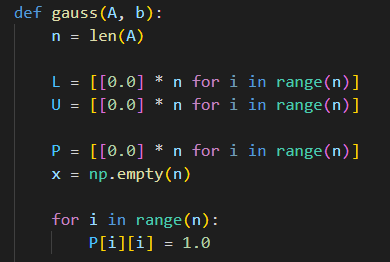
\includegraphics[height=6cm, width=12cm]{initialization.png}
\\
\normalsize{Η συνάρτηση καλείται με ορίσματα τους πίνακες \lt
A[nxn] \gt και \lt b[n]. \gt Παίρνουμε το μέγεθος του πίνακα και
αρχικοποιούμε τους πίνακες \lt L[nxn], U[nxn], P[nxn], x[n].  \gt
Οι πίνακες \lt L, P \gt αρχικοποιούνται ως μοναδιαίοι ενώ οι άλλοι ως
μηδενικοί. Στόχος είναι να λύσουμε την γραμμική σχέση:}
\\
\begin{equation*}
	Ax = b
\end{equation*}
\\
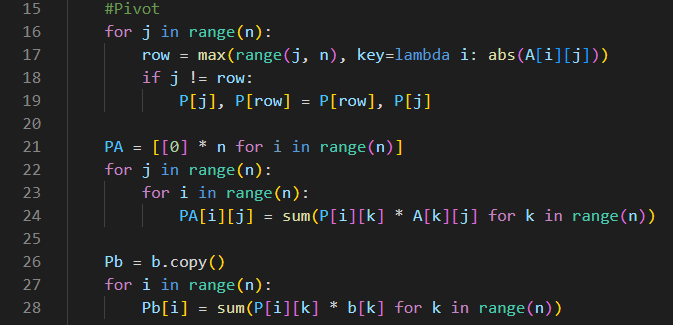
\includegraphics[height=6.5cm, width=12cm]{pivot.png}
\\
\normalsize{Αρχικά πραγματοποιούμε την οδήγηση. Δηλαδή ελέγχουμε κάθε
στήλη του πίνακα Α ώστε να βρούμε το μεγαλύτερο κατ'απόλυτη τιμή
στοιχείο της στήλης \lt j \gt και αντιμεταθέτουμε την γραμμή 
\lt j \gt με τη γραμμή που περιέχει το συγκεκριμένο στοιχείο. 
Αφού γίνει αυτό πολλαπλασιάζουμε τον πίνακα \lt A \gt και \lt b
\gt με τον πίνακα μετάβασης \lt P.}
\\
\begin{equation*}
	PAx = Pb
\end{equation*}
\\
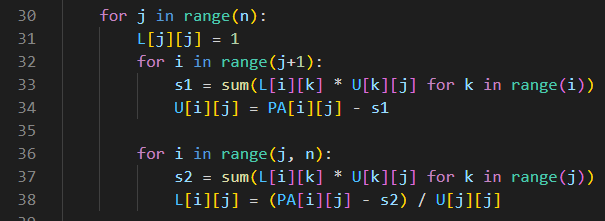
\includegraphics[height=6cm, width=12cm]{LU.png}
\\
\normalsize{Στη συνέχεια, υπολογίζουμε τους άνω και κάτω τριγωνικους
πίνακες \lt U, L \gt με τους εξής τύπους:}	
\\
\begin{equation*}
U_{ij} = PA_{ij}-\sum_{k=0}^{i-1}L_{ik}U_{kj}
\end{equation*}
\begin{equation*}
L_{ij} = \frac{(PA_{ij}-\sum_{k=0}^{i-1}L_{ik}U_{kj})}{U_{jj}}
\end{equation*}
\\
\normalsize{Και φτιάχνουμε την σχέση}
\\
\begin{equation*}
	LU = PA => LUx = Pb
\end{equation*}
\\
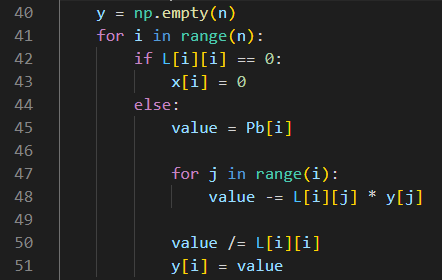
\includegraphics[height=6cm, width=12cm]{y.png}
\\
\normalsize{Λύνουμε πρώτα την σχέση}
\\
\begin{equation*}
	Ly = Pb
\end{equation*}
\\
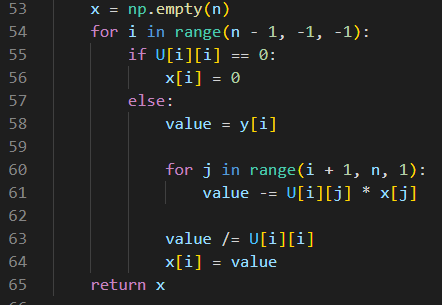
\includegraphics[height=6cm, width=12cm]{x.png}
\\
\normalsize{Ύστερα την σχέση}
\\
\begin{equation*}
	Ux = y
\end{equation*}
\\
\normalsize{Και η συνάρτηση μας επιστρέφει την λύση \lt x}
\subsection{\lt Cholesky}
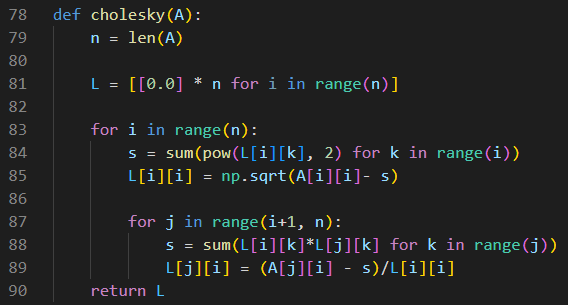
\includegraphics[height=6cm, width=12cm]{cholesky.png}
\\
\normalsize{Η συνάρτηση καλείται με ορίσμα έναν συμμετρικό και
θετικά ορισμένο πίνακα \lt
A[nxn]. \gt Παίρνουμε το μέγεθος\lt (n) \gt του πίνακα και
αρχικοποιούμε τον πίνακα \lt L[nxn] \gt ως μηδενικό. Στην συνέχεια,
εφαρμόζουμε τους παρακάτω τύπους του αλγορίθμου \lt Cholesky.} 
\\
	\begin{equation*}
L_{ii} = \sqrt{A_{ii}-\sum_{k=0}^{i-1}L^2_{ik}}
	\end{equation*}	
	\begin{equation*}
L_{ji} = \frac{1}{L_{ii}}(A_{ij}-\sum_{k=0}^{j-1}L_{ik}L_{jk}), 
    \; \;  for \; j>i
	\end{equation*}
	\normalsize{Στο τέλος η συνάρτηση επιστρέφει τον πίνακα \lt L.}

	\subsection{\lt Gauss-Seidel}
	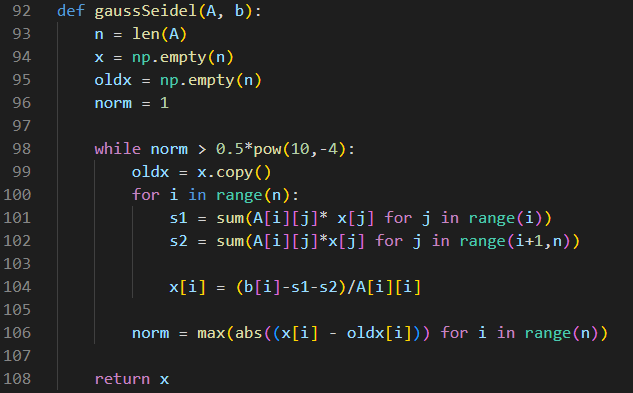
\includegraphics[height=7cm, width=12cm]{gauss-seidel.png}

	\normalsize{Η συνάρτηση καλείται με ορίσματα τους πίνακες \lt\\
A[nxn] \gt και \lt b[n]. \gt 
Παίρνουμε το μέγεθος\lt (n) \gt του πίνακα, ορίζουμε την νόρμα 
\lt (norm) \gt με 1 και
αρχικοποιούμε τους πίνακες \lt x[n], oldx[n] \gt ως μηδενικούς.
Στην συνέχεια, όσο ισχύει}
\begin{equation*}
norm = ||x - oldx|| > 0,5*10^{-4}
\end{equation*}
\normalsize{αποθηκεύουμε το \lt x \gt στο \lt oldx \gt και 
εφαρμόζουμε τον παρακάτω τύπο του αλγορίθμου \lt Gauss-Seidel.}
\begin{equation*}
x^{k+1}_i = \frac{b_i - \sum_{j=0}^{i-1} a_{ij} x_j^{k+1} -
\sum_{j=i+1}^{n-1} a_{ij} x^k_j}{a_{ii}}
\end{equation*}
\normalsize{Τελικά, η συνάρτηση επιστρέφει τον πίνακα 
\lt x \gt που είναι η προσεγγιστική λύση.
\\ Για τον πίνακα Α με το μάτι καταλαβαίνουμε ότι η λύση είναι
\\ \lt x = [1, 1, ..., 1]
\\ \gt Άρα θα εξετάσουμε αν κάθε στοιχείο της \lt x \gt
απέχει στο 1 λιγότερο από το σφάλμα.}
\\
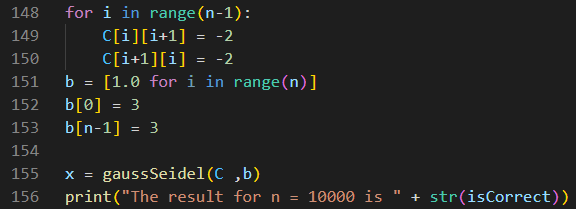
\includegraphics[height=4cm, width=12cm]{result.png}
\\
\normalsize{\lt The result for n = 10 is True
\\The result for n = 10000 is True}


\section{Άσκηση 4}
	\subsection{Απόδειξη ότι ο \lt G \gt είναι στοχαστικός}
\normalsize{Στοχαστικός πίνακας ονομάζεται ένας τετραγωνικός
πίνακας με μη αρνητικά στοιχεία τα οποία αναπαριστούν πιθανότητες.
Οι γραμμές (ή οι στήλες) του έχουν άθροισμα 1. Άρα πρέπει να
αποδείξουμε ότι το άθροισμα των γραμμών (ή των στηλών του) έχει
άθροισμα 1.}
\\
\begin{equation*}
\sum_{j = 0}^{n-1}Gij = \sum_{j = 0}^{n-1} (\frac{q}{n} +
\frac{A_{ij}(1-q)}{n_j})
= \frac{nq}{n} + \frac{1-q}{n_j}\sum_{j = 0}^{n-1}A_{ij} =
\end{equation*}
\begin{equation*}
q + \frac{(1-q)n_j}{n_j} = q + 1 -q = 1
\end{equation*}
\normalsize{Άρα ο πίνακας είναι στοχαστικός γιατί οι στήλες του έχουν
άθροισμα 1.}
	\subsection{\lt p = Gp}
	\normalsize{\lt G =} 
\begin{equation*}
\hspace{-3cm}	
\setcounter{MaxMatrixCols}{20}
\begin{pmatrix}
0.01 & 0.01 & 0.01 & 0.01 & 0.435 & 0.01 & 0.01 & 0.01 & 0.01 & 0.01 & 0.01 & 0.01 & 0.01 & 0.01 & 0.01 \\
        0.435 & 0.01 & 0.2933 & 0.01 & 0.01 & 0.01 & 0.01 & 0.01 & 0.01 & 0.01 & 0.01 & 0.01 & 0.01 & 0.01 & 0.01 \\
        0.01 & 0.2933 & 0.01 & 0.435 & 0.01 & 0.01 & 0.01 & 0.01 & 0.01 & 0.01 & 0.01 & 0.01 & 0.01 & 0.01 & 0.01 \\
        0.01 & 0.01 & 0.01 & 0.01 & 0.01 & 0.01 & 0.01 & 0.435 & 0.01 & 0.01 & 0.01 & 0.01 & 0.01 & 0.01 & 0.01 \\
        0.01 & 0.2933 & 0.01 & 0.01 & 0.01 & 0.01 & 0.01 & 0.01 & 0.2933 & 0.01 & 0.01 & 0.01 & 0.01 & 0.01 & 0.01 \\
        0.01 & 0.01 & 0.2933 & 0.01 & 0.01 & 0.01 & 0.01 & 0.01 & 0.2933 & 0.01 & 0.01 & 0.01 & 0.01 & 0.01 & 0.01 \\
        0.01 & 0.2933 & 0.01 & 0.01 & 0.01 & 0.01 & 0.01 & 0.01 & 0.01 & 0.01 & 0.01 & 0.2933 & 0.01 & 0.01 & 0.01 \\
        0.01 & 0.01 & 0.2933 & 0.01 & 0.01 & 0.01 & 0.01 & 0.01 & 0.01 & 0.01 & 0.01 & 0.2933 & 0.01 & 0.01 & 0.01 \\
        0.435 & 0.01 & 0.01 & 0.01  &0.01 & 0.01 & 0.01 & 0.01 & 0.01 & 0.01 & 0.01 & 0.01 & 0.435 & 0.01 & 0.01 \\
        0.01 & 0.01 & 0.01 & 0.01 & 0.435 & 0.435 & 0.435 & 0.01 & 0.2933 & 0.01 & 0.01 & 0.01 & 0.01 & 0.2225 & 0.01\\ 
        0.01 & 0.01 & 0.01 & 0.01 & 0.01 & 0.435 & 0.435 & 0.435 & 0.01 & 0.01 & 0.01 & 0.2933 & 0.01 & 0.2225 & 0.01 \\
        0.01 & 0.01 & 0.01 & 0.435 & 0.01 & 0.01 & 0.01 & 0.01 & 0.01 & 0.01 & 0.01 & 0.01 & 0.01 & 0.01 & 0.435 \\
        0.01 & 0.01 & 0.01 & 0.01 & 0.01 & 0.01 & 0.01 & 0.01 & 0.01 & 0.86 & 0.01 & 0.01 & 0.01 & 0.2225 & 0.01 \\
        0.01 & 0.01 & 0.01 & 0.01 & 0.01 & 0.01 & 0.01 & 0.01 & 0.01 & 0.01 & 0.01 & 0.01 & 0.435 & 0.01 & 0.435 \\
0.01 & 0.01 & 0.01 & 0.01 & 0.01 & 0.01 & 0.01 & 0.01 & 0.01 & 0.01 & 0.86 & 0.01 & 0.01 & 0.2225 & 0.01

\end{pmatrix}
\end{equation*}
\normalsize{Το πρόγραμμα βρίσκει με την μέθοδο των δυνάμεων για
ακρίβεια 10\lt e-5 \gt το ιδιοδυάνισμα 

\lt p = [0.02682389, 0.02986128, 0.02986128, 0.02682389, 0.03958766,
...\\
0.03958766, 0.03958766, 0.03958766, 0.07456589, 0.10631849, ...\\
0.10631849, 0.07456589, 0.12508977, 0.11633074, 0.12508977]
\\ 
\gt το οποίο είναι περίπου ίδιο με το ιδιοδυάνισμα που μας δίνεται}

	
	\subsection{Βελτίωση βαθμού σημαντικότητας}
\normalsize{Διαλέγω να βελτιώσω τον βαθμό σημαντικότητας της πρώτης
σελίδας. Οπότε προσθέτω συνδέσεις από την δεύτερη, τρίτη, τέταρτη και
έκτη σελίδα (Η πέμπτη ήδη πάει στην πρώτη). Αφαιρώ τυχαία την σύνδεση
της τρίτης στην δεύτερη. Το αποτέλεσμα είναι:
\\p = [0.06184402 0.0362909  0.02482734 0.02509765 0.04261679 ...
\\0.04193646 0.03621257 0.03553223 0.08790694 0.10360136  ...
\\0.09418914 0.06532107 0.12139946 0.10982291 0.11340116]
\\Βλέπουμε ότι ο βαθμός σημαντικότητας της πρώτης σελίδας έχει
σχεδόν τριπλασιαστεί}

	\subsection{Αλλαγή πιθανότητας μεταπήδησης}
		\subsubsection{\lt q = 0.02}
\normalsize{\lt Result for q = 0.02 in 4.4(A) is: \\
p = [0.04614265 0.02394582 0.01210989 0.01502407 0.03760068 
\\0.0356886 0.02985731 0.02794523 0.09306153 0.10916014 
\\0.09668641 0.06936467 0.1410327  0.1335713  0.12880899]}
		\subsubsection{\lt q = 0.6}
\normalsize{\lt Result for q = 0.6 in 4.4(B) is: \\
p = [0.07792531 0.05558503 0.05236878 0.05107864 0.05514962
\\ 0.05657374 0.05396778 0.05539189 0.07193381 0.08621975
\\ 0.0850861  0.06306842 0.08174926 0.07260688 0.08129499]}
\\
\normalsize{Ο σκοπός της πιθανότητας μεταπήδησης είναι να 
χαρακτηρίζει πόσο σημαντικό είναι μια σελίδα να δέχεται συνδέσμους
από άλλες σελίδες. Όσο μικρότερο τόσο σημαντικότερο και το
αντίστροφο. Βλέπουμε επίσης ότι για μεγάλο \lt q 
\gt όλες οι σελίδες έχουν
μικρότερες διαφορές στις τάξεις τους}

	\subsection{Βελτίωση τάξης της σελίδας 11}
\normalsize{\lt
Result for 4.5(before) is:
\\ Rank of 11 = 0.10631848768394055
\\ Rank of 10 = 0.10631848768394055
\\ Result for 4.5(after) is:
\\ Rank of 11 = 0.12400835065568959
\\ Rank of 10 = 0.10289405307708084
\\ \gt Όντως αυτή η στρατηγική δουλεύει}	
	
	\subsection{Διαγραφή της σελίδας 10}
\normalsize{\lt 
Difference after deletion of site 10 for 4.6 is
\\ diff = [0.0446, 0.0314, 0.0314, 0.0142, 0.0217, 0.0217, 0.0116,
0.0116, -0.0031, 0, -0.0031, -0.0941, -0.0449, -0.0334]
\\ \gt Παρατηρούμε ότι οι τάξεις σελιδών που αυξάνονται είναι αυτές
με μεγάλο βαθμό σημαντικότητας ενώ μειώνονται οι σελίδες με μικρό
βαθμό}

\end{document}